\documentclass[a4paper,12pt]{article}

% Ελληνικά
\usepackage[utf8]{inputenc}
\usepackage[greek,english]{babel}
\usepackage{alphabeta}

% Μαθηματικά
\usepackage{amsmath,amssymb,amsfonts}

% Γραφικά & Πίνακες
\usepackage{graphicx}
\usepackage{float}
\usepackage{booktabs}
\usepackage{array}
\usepackage{multirow}
\usepackage{longtable}
\usepackage{tabularx}

% Μορφοποίηση
\usepackage[margin=2.5cm]{geometry}
\usepackage{setspace}
\onehalfspacing
\usepackage{parskip}
\usepackage{enumitem}
\usepackage{fancyhdr}
\usepackage{titlesec}
\usepackage{xcolor}
\usepackage{tcolorbox}
\usepackage{hyperref}

% Χρώματα
\definecolor{decisiongreen}{RGB}{76,175,80}
\definecolor{chanceorange}{RGB}{255,152,0}
\definecolor{resultblue}{RGB}{33,150,243}

% Κεφαλίδες
\pagestyle{fancy}
\fancyhf{}
\rhead{Εργασία 3 -- Ανάλυση Αποφάσεων}
\lhead{ΠΜΣ Υπολ. \& Στατ. Αναλυτική}
\cfoot{\thepage}

\hypersetup{colorlinks=true,linkcolor=blue,urlcolor=blue}

\begin{document}

% ============================================================================
% ΤΙΤΛΟΣ
% ============================================================================
\begin{titlepage}
\centering
\vspace*{2cm}

{\LARGE\bfseries Πανεπιστήμιο -- ΠΜΣ: Υπολογιστική και Στατιστική\\Αναλυτική στην Επιστήμη των Δεδομένων}

\vspace{1cm}

{\Large Μάθημα: Ανάλυση Αποφάσεων και Βελτιστοποίηση}

\vspace{0.5cm}

{\large Διδάσκων: Ν. Τσάντας}

\vspace{2cm}

{\Huge\bfseries Εργασία 3}

\vspace{1cm}

{\Large Ακαδημαϊκό Έτος: 2025--26}

\vspace{3cm}

{\Large\bfseries Όνομα Φοιτητή: [Συμπληρώστε]}

\vspace{0.5cm}

{\large ΑΜ: [Συμπληρώστε]}

\vfill

{\large Φεβρουάριος 2026}
\end{titlepage}

\tableofcontents
\newpage

% ============================================================================
% ΑΣΚΗΣΗ 1A: Chelsea Bush
% ============================================================================
\section{Μικρή Άσκηση: Chelsea Bush (Άσκηση A)}

\subsection{Εννοιολογική Προσέγγιση}

Η Chelsea Bush είναι υποψήφια για το χρίσμα του κόμματός της για την Προεδρία των ΗΠΑ. Αντιμετωπίζει μια ακολουθία αποφάσεων σχετικά με τη συμμετοχή της στα προκριματικά:

\begin{itemize}
    \item \textbf{1η Απόφαση}: Να συμμετάσχει ή όχι στα προκριματικά του New Hampshire (N.H.)
    \item \textbf{2η Απόφαση}: Ανάλογα με το αποτέλεσμα, να συμμετάσχει ή όχι στα Super Tuesday (S.T.)
\end{itemize}

\textbf{Στόχος}: Μεγιστοποίηση των αναμενόμενων διαθέσιμων κεφαλαίων μετά τα προκριματικά.

\textbf{Δεδομένα:}
\begin{itemize}
    \item $P(\text{Καλά S.T.}) = 0.4$, \quad $P(\text{Άσχημα S.T.}) = 0.6$
    \item Κέρδος αν πάει καλά στο S.T.: \$16 εκατ., Ζημία αν πάει άσχημα: \$10 εκατ.
    \item $P(\text{Καλά S.T.} \mid \text{Καλά N.H.}) = 4/7$
    \item $P(\text{Καλά S.T.} \mid \text{Άσχημα N.H.}) = 1/7$
    \item $P(\text{Καλά N.H.}) = 7/15$
    \item Κόστος εκστρατείας N.H.: \$1.6 εκατ.
\end{itemize}

\subsection{Μοντέλο και Λύση}

\subsubsection{Ανάλυση Δέντρου Απόφασης}

\textbf{Κλαδί Α: Χωρίς συμμετοχή στο N.H.}

Αν η Chelsea δεν συμμετάσχει στο N.H., η απόφαση για το S.T. βασίζεται στις αρχικές πιθανότητες:
\begin{align}
EV(\text{Συμμ. S.T.}) &= P(\text{Καλά}) \times 16 + P(\text{Άσχημα}) \times (-10) \nonumber \\
&= 0.4 \times 16 + 0.6 \times (-10) = 6.4 - 6.0 = \mathbf{\$0.40 \text{ εκατ.}}
\end{align}

Αφού $EV(\text{Συμμ. S.T.}) = \$0.40\text{M} > 0 = EV(\text{Μη Συμμ.})$, η βέλτιστη απόφαση είναι \textbf{συμμετοχή στο S.T.} με $EV = \$0.40$ εκατ.

\textbf{Κλαδί Β: Με συμμετοχή στο N.H.}

\underline{Αν τα πάει καλά στο N.H.:}
\begin{align}
EV(\text{Συμμ. S.T.} \mid \text{Καλά N.H.}) &= \frac{4}{7} \times 16 + \frac{3}{7} \times (-10) \nonumber \\
&= \frac{64}{7} - \frac{30}{7} = \frac{34}{7} \approx \mathbf{\$4.857 \text{ εκατ.}}
\end{align}
Αφού $4.857 > 0$: \textbf{Συμμετοχή στο S.T.}

\underline{Αν τα πάει άσχημα στο N.H.:}
\begin{align}
EV(\text{Συμμ. S.T.} \mid \text{Άσχημα N.H.}) &= \frac{1}{7} \times 16 + \frac{6}{7} \times (-10) \nonumber \\
&= \frac{16}{7} - \frac{60}{7} = -\frac{44}{7} \approx \mathbf{-\$6.286 \text{ εκατ.}}
\end{align}
Αφού $-6.286 < 0$: \textbf{Μη συμμετοχή στο S.T.}

\underline{Συνολική αξία συμμετοχής στο N.H.:}
\begin{align}
EV(\text{N.H.}) &= P(\text{Καλά N.H.}) \times EV^*(\text{Καλά}) + P(\text{Άσχημα N.H.}) \times EV^*(\text{Άσχημα}) - \text{Κόστος} \nonumber \\
&= \frac{7}{15} \times \frac{34}{7} + \frac{8}{15} \times 0 - 1.6 \nonumber \\
&= \frac{34}{15} - 1.6 = 2.267 - 1.6 = \mathbf{\$0.667 \text{ εκατ.}}
\end{align}

\subsubsection{Βέλτιστη Πολιτική}

\begin{tcolorbox}[colback=green!10, colframe=decisiongreen, title=Βέλτιστη Πολιτική]
\begin{enumerate}
    \item \textbf{Συμμετοχή στο N.H.} (EV = \$0.667M $>$ \$0.40M χωρίς N.H.)
    \item Αν \textbf{καλά στο N.H.} $\rightarrow$ \textbf{Συμμετοχή στο S.T.}
    \item Αν \textbf{άσχημα στο N.H.} $\rightarrow$ \textbf{Μη συμμετοχή στο S.T.}
\end{enumerate}
Αναμενόμενα κεφάλαια: \textbf{\$666,667}
\end{tcolorbox}

\begin{figure}[H]
    \centering
    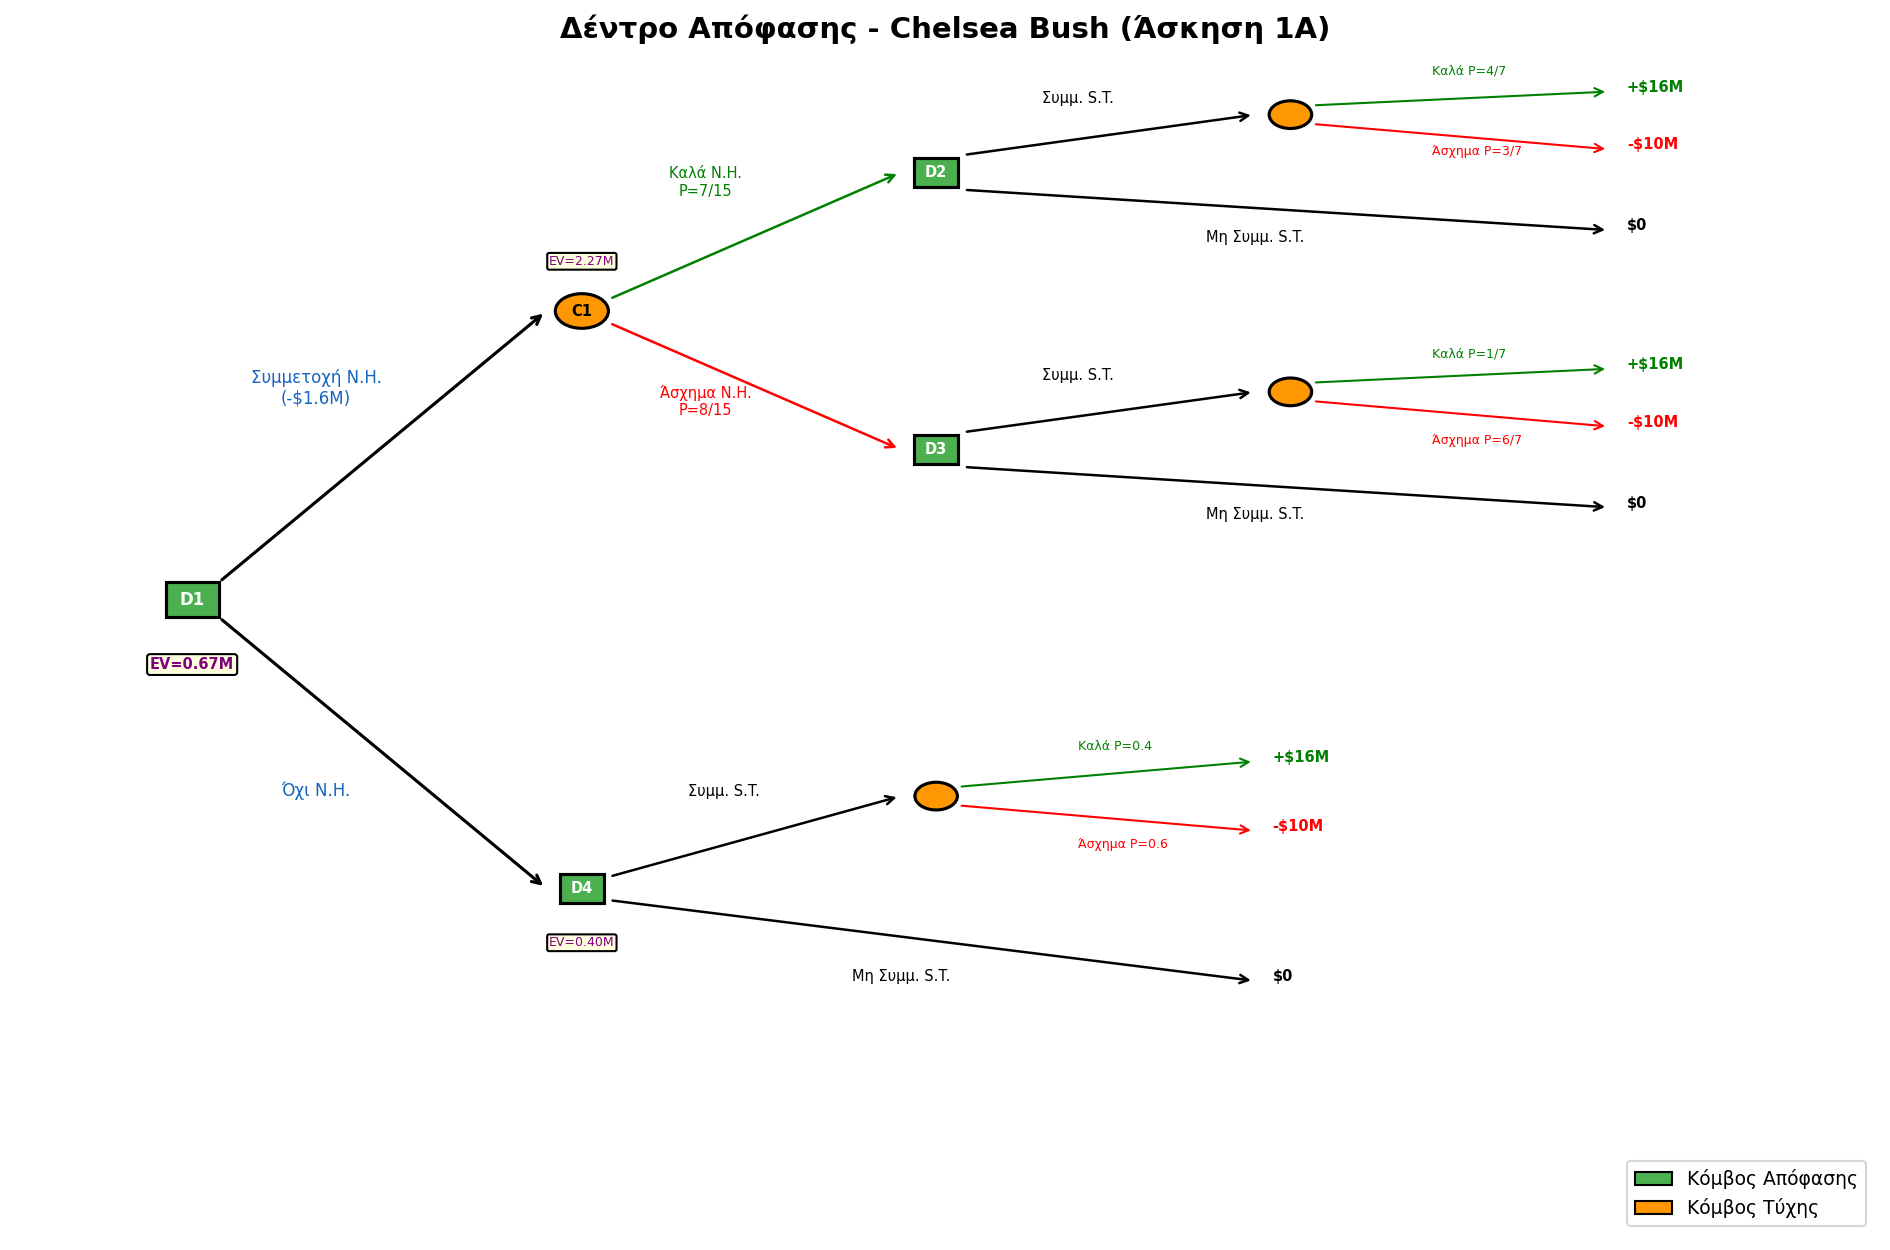
\includegraphics[width=\textwidth]{figures/ex1a_tree.png}
    \caption{Δέντρο Απόφασης -- Chelsea Bush}
\end{figure}

\subsubsection{Ανάλυση Ευαισθησίας (Μέρος b)}

Εξετάζουμε πώς μεταβάλλεται η αναμενόμενη αποδοχή όταν τα ποσά κέρδους (\$16M) και ζημίας (\$10M) μεταβάλλονται κατά $\pm25\%$.

\textbf{Εύρος μεταβολής:}
\begin{itemize}
    \item Κέρδος: \$12M -- \$20M (βασικό: \$16M)
    \item Ζημία: \$7.5M -- \$12.5M (βασικό: \$10M)
\end{itemize}

\begin{figure}[H]
    \centering
    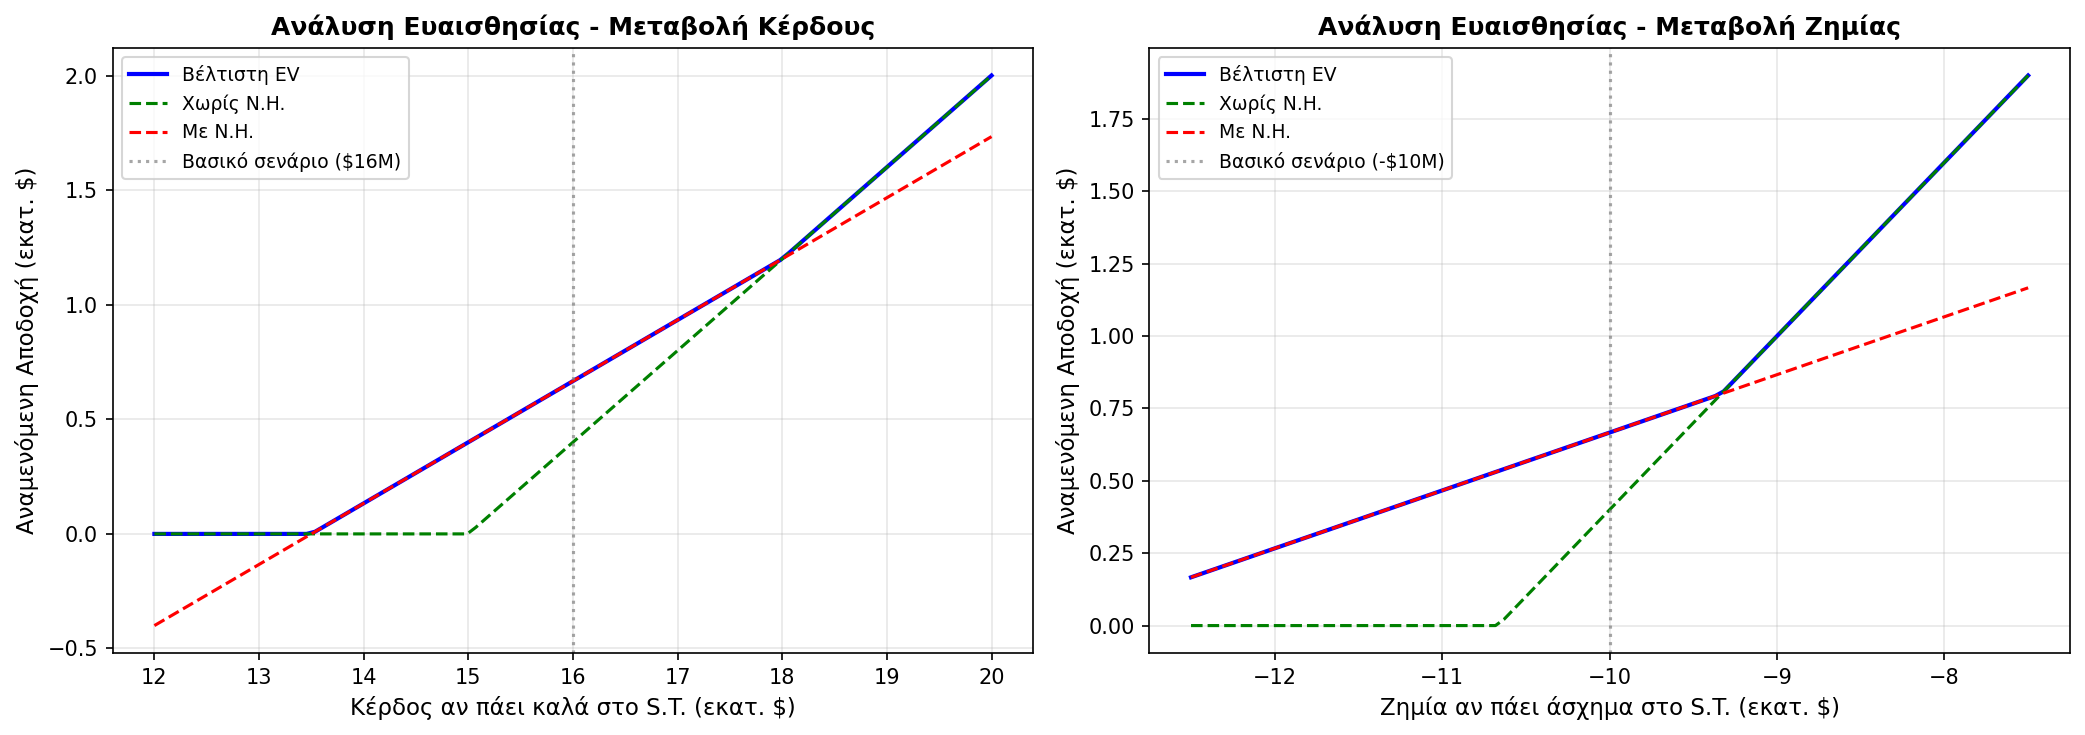
\includegraphics[width=\textwidth]{figures/ex1a_sensitivity.png}
    \caption{Ανάλυση Ευαισθησίας -- Μεταβολή κέρδους και ζημίας}
\end{figure}

Η ανάλυση δείχνει ότι η στρατηγική με N.H. παραμένει βέλτιστη σε ολόκληρο το εύρος μεταβολής. Η πληροφορία από το N.H. προσφέρει σταθερό πλεονέκτημα διότι επιτρέπει την αποφυγή ζημιογόνων αποφάσεων.


% ============================================================================
% ΑΣΚΗΣΗ 2: Steeley Associates
% ============================================================================
\newpage
\section{Steeley Associates, Inc.}

\subsection{Εννοιολογική Προσέγγιση}

Η Steeley Associates κατέχει ένα ιστορικό ακίνητο και αντιμετωπίζει τρεις αρχικές επιλογές:
\begin{enumerate}
    \item \textbf{Πώληση ακινήτου}: Εγγυημένα \$900,000
    \item \textbf{Κατασκευή κτιρίου γραφείων}: Εξαρτάται από ανάπτυξη πόλης
    \item \textbf{Αίτηση άδειας διαμερισμάτων}: Σειρά πιθανών εκβάσεων
\end{enumerate}

Το πρόβλημα περιλαμβάνει πολλαπλά στάδια αποφάσεων με ενδεχόμενη δικαστική διαμάχη.

\subsection{Μοντέλο και Λύση}

\subsubsection{Βήμα 1: Πώληση ακινήτου}
\[
EV(\text{Πώληση}) = \$900{,}000
\]

\subsubsection{Βήμα 2: Κτίριο γραφείων}
\begin{align}
EV(\text{Γραφεία}) &= 0.70 \times \$1{,}300{,}000 + 0.30 \times \$200{,}000 \nonumber \\
&= \$910{,}000 + \$60{,}000 = \mathbf{\$970{,}000}
\end{align}

\subsubsection{Βήμα 3: Αίτηση άδειας (backward induction)}

\textbf{Αν η Steeley χάσει τη μήνυση:}
\begin{align}
EV(\text{Πώληση μετά ήττα}) &= 0.50 \times \$900{,}000 + 0.50 \times \$500{,}000 = \$700{,}000 \\
EV(\text{Γραφεία μετά ήττα}) &= 0.50 \times \$1{,}200{,}000 + 0.50 \times \$100{,}000 = \$650{,}000
\end{align}
Βέλτιστη: \textbf{Πώληση} με $EV = \$700{,}000$

\textbf{Αξιολόγηση μήνυσης:}
\begin{align}
EV(\text{Μήνυση}) &= 0.40 \times (\$1{,}000{,}000 + \$3{,}000{,}000) + 0.10 \times (-\$200{,}000) \nonumber \\
&\quad + 0.50 \times \$700{,}000 - \$300{,}000 \nonumber \\
&= \$1{,}600{,}000 - \$20{,}000 + \$350{,}000 - \$300{,}000 = \mathbf{\$1{,}630{,}000}
\end{align}

\textbf{Μετά απόρριψη άδειας:}
\begin{itemize}
    \item Πώληση: \$700,000
    \item Γραφεία: \$970,000
    \item Μήνυση: \$1,630,000 $\leftarrow$ \textbf{Βέλτιστη}
\end{itemize}

\textbf{Αξιολόγηση αίτησης άδειας:}
\begin{align}
EV(\text{Αίτηση}) &= 0.10 \times \$3{,}000{,}000 + 0.90 \times \$1{,}630{,}000 \nonumber \\
&= \$300{,}000 + \$1{,}467{,}000 = \mathbf{\$1{,}767{,}000}
\end{align}

\subsubsection{Τελική Σύγκριση}

\begin{table}[H]
\centering
\begin{tabular}{lrr}
\toprule
\textbf{Επιλογή} & \textbf{EV (\$)} & \textbf{Κατάταξη} \\
\midrule
Πώληση ακινήτου & 900,000 & 3η \\
Κτίριο γραφείων & 970,000 & 2η \\
\textbf{Αίτηση άδειας} & \textbf{1,767,000} & \textbf{1η} \\
\bottomrule
\end{tabular}
\caption{Σύγκριση εναλλακτικών -- Steeley Associates}
\end{table}

\begin{tcolorbox}[colback=green!10, colframe=decisiongreen, title=Βέλτιστη Πολιτική -- Steeley Associates]
\begin{enumerate}
    \item \textbf{Αίτηση άδειας διαμερισμάτων}
    \item Αν εγκριθεί (10\%) $\rightarrow$ Κατασκευή διαμερισμάτων (\$3M)
    \item Αν απορριφθεί (90\%) $\rightarrow$ \textbf{Μήνυση δήμου} (-\$300K δικ. έξοδα)
    \begin{itemize}
        \item Αν κερδίσει (40\%) $\rightarrow$ \$4M
        \item Αν εκκρεμεί (10\%) $\rightarrow$ -\$200K
        \item Αν χάσει (50\%) $\rightarrow$ \textbf{Πώληση ακινήτου}
    \end{itemize}
\end{enumerate}
Αναμενόμενη αξία: \textbf{\$1,767,000}
\end{tcolorbox}

\begin{figure}[H]
    \centering
    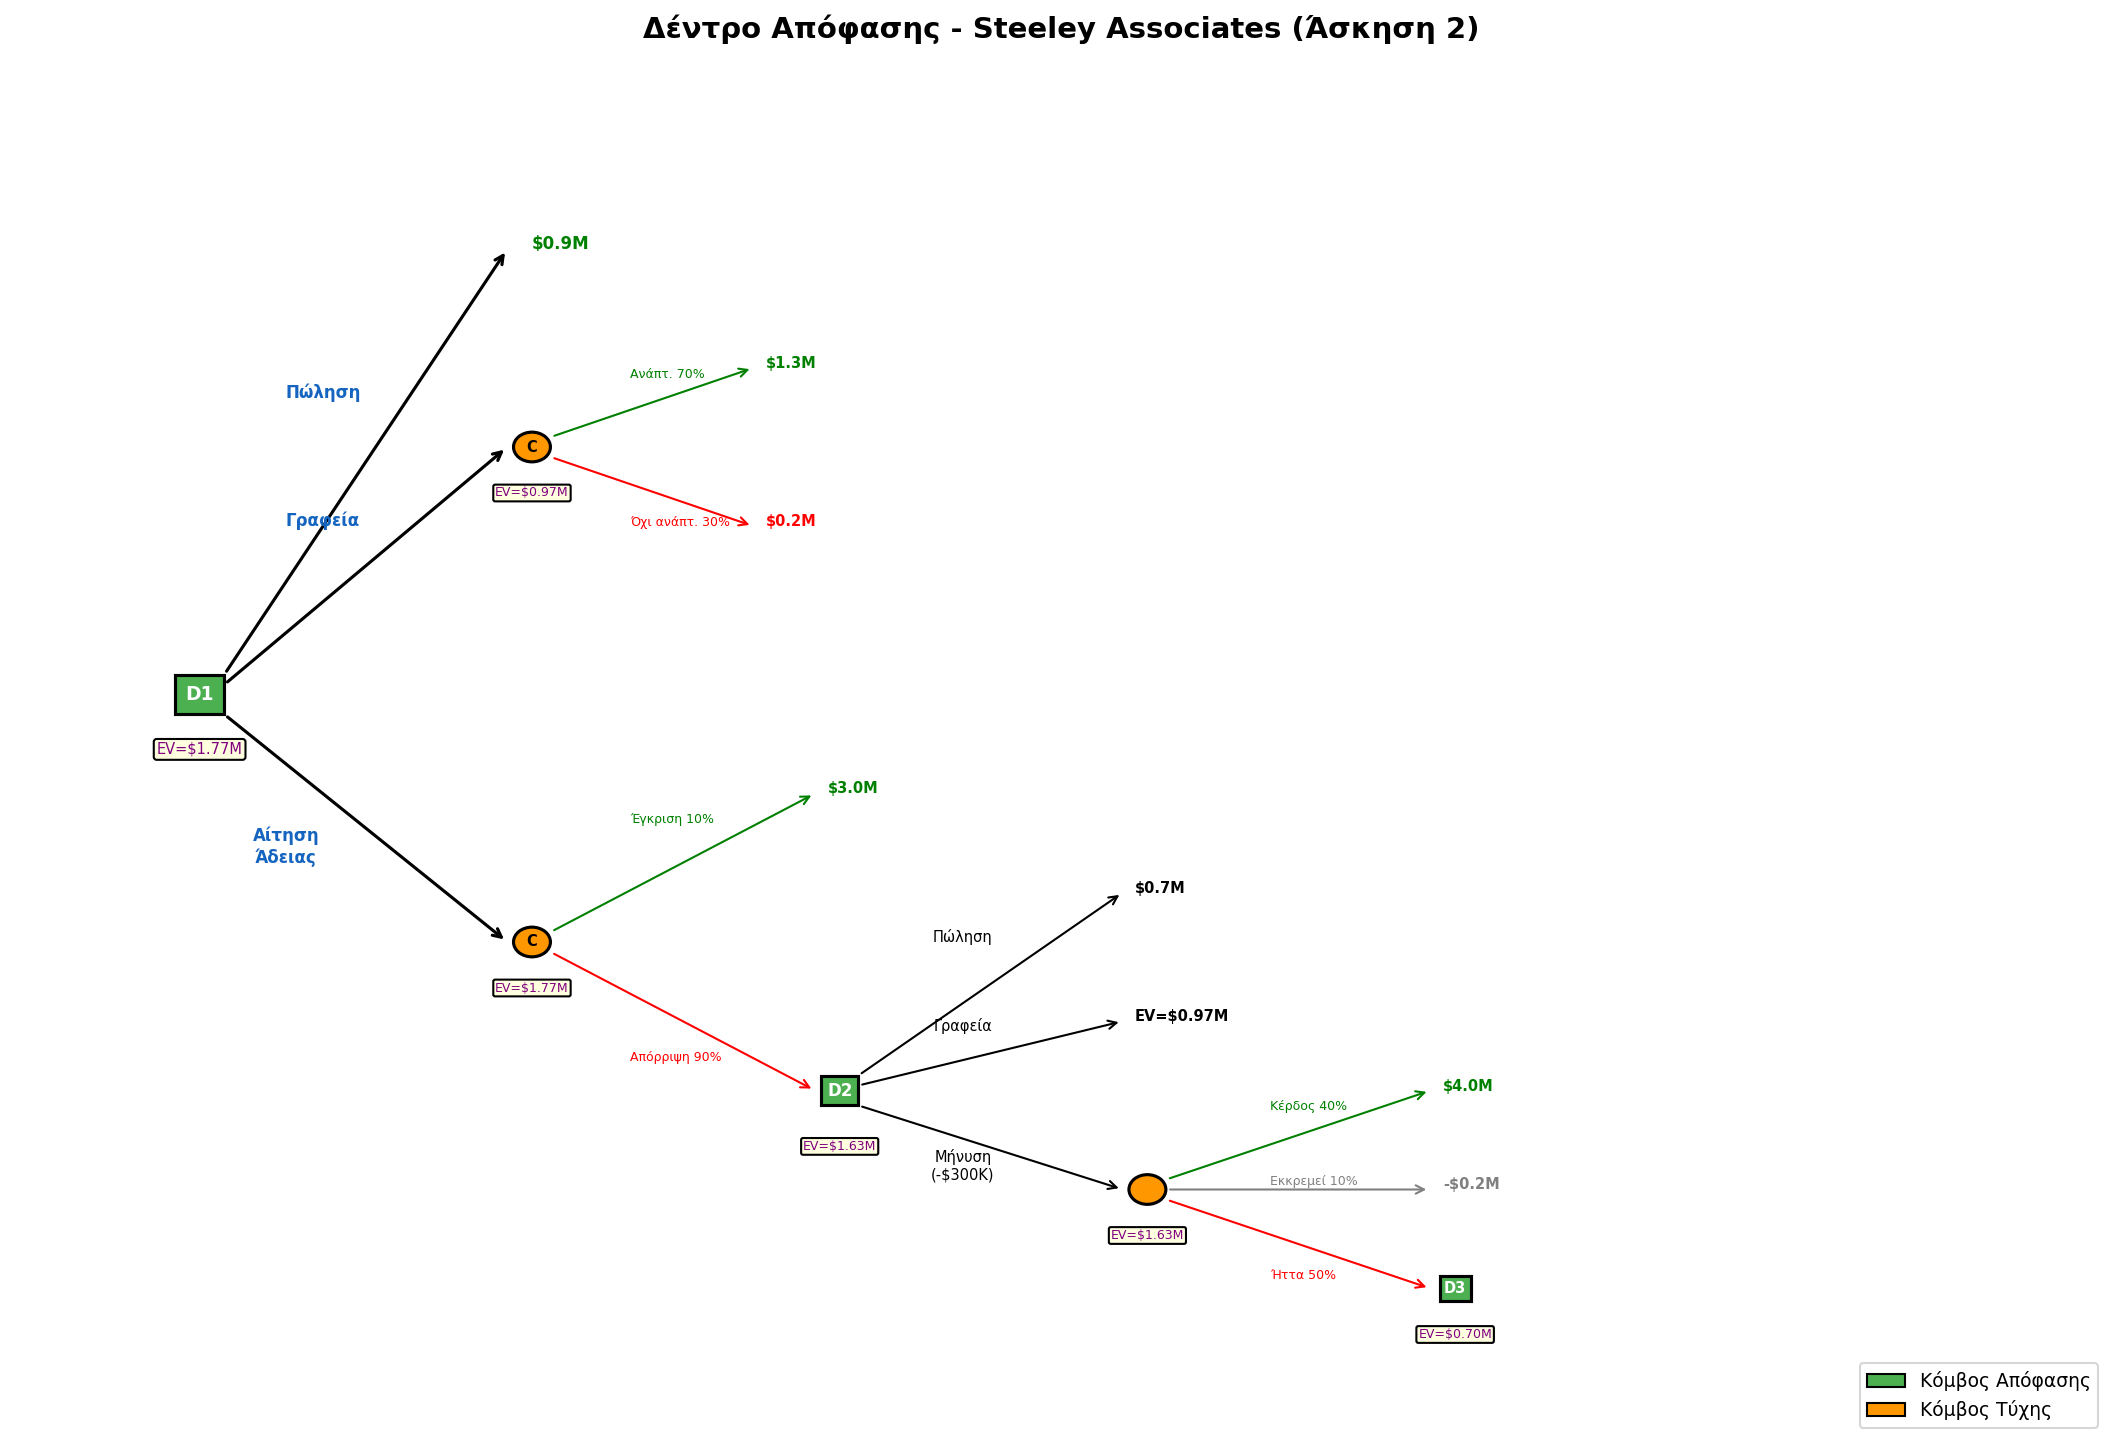
\includegraphics[width=\textwidth]{figures/ex2_steeley_tree.png}
    \caption{Δέντρο Απόφασης -- Steeley Associates}
\end{figure}


% ============================================================================
% ΑΣΚΗΣΗ 3: BAAG/DSS
% ============================================================================
\newpage
\section{Smart Steering Support (BAAG/DSS)}

\subsection{Εννοιολογική Προσέγγιση}

Η εταιρεία Bay Area Automobile Gadgets (BAAG) εξετάζει την ανάπτυξη ενός συστήματος υποστήριξης οδηγού (DSS) με ενσωματωμένη συσκευή σάρωσης δρόμου. Το πρόβλημα περιλαμβάνει αλληλουχία αποφάσεων:

\begin{enumerate}
    \item \textbf{D1}: Επένδυση στην έρευνα (\$300K) ή πώληση DSS ως έχει (\$2M)
    \item \textbf{D2}: Αν η έρευνα επιτύχει: Ανάπτυξη προϊόντος (\$800K) ή πώληση τεχνολογίας στη GM (\$200K + \$2M DSS)
    \item \textbf{D3}: Αν η ανάπτυξη επιτύχει: Κυκλοφορία στην αγορά (\$200K) ή πώληση concept στη GM (\$1M)
\end{enumerate}

\subsection{Μοντέλο και Λύση}

\subsubsection{Backward Induction -- Βήμα 1: Αποδοχή Αγοράς}

\begin{align}
EV(\text{Αγορά}) &= 0.30 \times \$8{,}000{,}000 + 0.50 \times \$4{,}000{,}000 + 0.20 \times \$2{,}200{,}000 \nonumber \\
&= \$2{,}400{,}000 + \$2{,}000{,}000 + \$440{,}000 = \mathbf{\$4{,}840{,}000}
\end{align}

\subsubsection{Βήμα 2: Απόφαση Κυκλοφορίας (D3)}

\begin{align}
EV(\text{Κυκλοφορία}) &= \$4{,}840{,}000 - \$200{,}000 = \$4{,}640{,}000 \\
EV(\text{Πώληση concept}) &= \$1{,}000{,}000
\end{align}
Βέλτιστη: \textbf{Κυκλοφορία} (\$4,640,000 $>$ \$1,000,000)

\subsubsection{Βήμα 3: Απόφαση Ανάπτυξης (D2)}

\begin{align}
EV(\text{Ανάπτυξη}) &= 0.65 \times \$4{,}640{,}000 + 0.35 \times \$2{,}200{,}000 - \$800{,}000 \nonumber \\
&= \$3{,}016{,}000 + \$770{,}000 - \$800{,}000 = \mathbf{\$2{,}986{,}000} \\
EV(\text{Μη Ανάπτ.}) &= \$2{,}000{,}000 + \$200{,}000 = \$2{,}200{,}000
\end{align}
Βέλτιστη: \textbf{Ανάπτυξη} (\$2,986,000 $>$ \$2,200,000)

\subsubsection{Βήμα 4: Απόφαση Έρευνας (D1)}

\begin{align}
EV(\text{Έρευνα}) &= 0.80 \times \$2{,}986{,}000 + 0.20 \times \$2{,}000{,}000 - \$300{,}000 \nonumber \\
&= \$2{,}388{,}800 + \$400{,}000 - \$300{,}000 = \mathbf{\$2{,}488{,}800} \\
EV(\text{Χωρίς Έρευνα}) &= \$2{,}000{,}000
\end{align}

\begin{tcolorbox}[colback=green!10, colframe=decisiongreen, title=Βέλτιστη Πολιτική -- BAAG/DSS]
\begin{enumerate}
    \item \textbf{Επένδυση στην Έρευνα} (-\$300K)
    \item Αν επιτυχής (80\%) $\rightarrow$ \textbf{Ανάπτυξη προϊόντος} (-\$800K)
    \begin{itemize}
        \item Αν επιτυχής (65\%) $\rightarrow$ \textbf{Κυκλοφορία στην αγορά} (-\$200K)
        \item Αν αποτυχία (35\%) $\rightarrow$ Πώληση DSS + τεχνολογίας (\$2.2M)
    \end{itemize}
    \item Αν αποτυχής (20\%) $\rightarrow$ Πώληση DSS (\$2M)
\end{enumerate}
Αναμενόμενη αξία: \textbf{\$2,488,800}
\end{tcolorbox}

\begin{figure}[H]
    \centering
    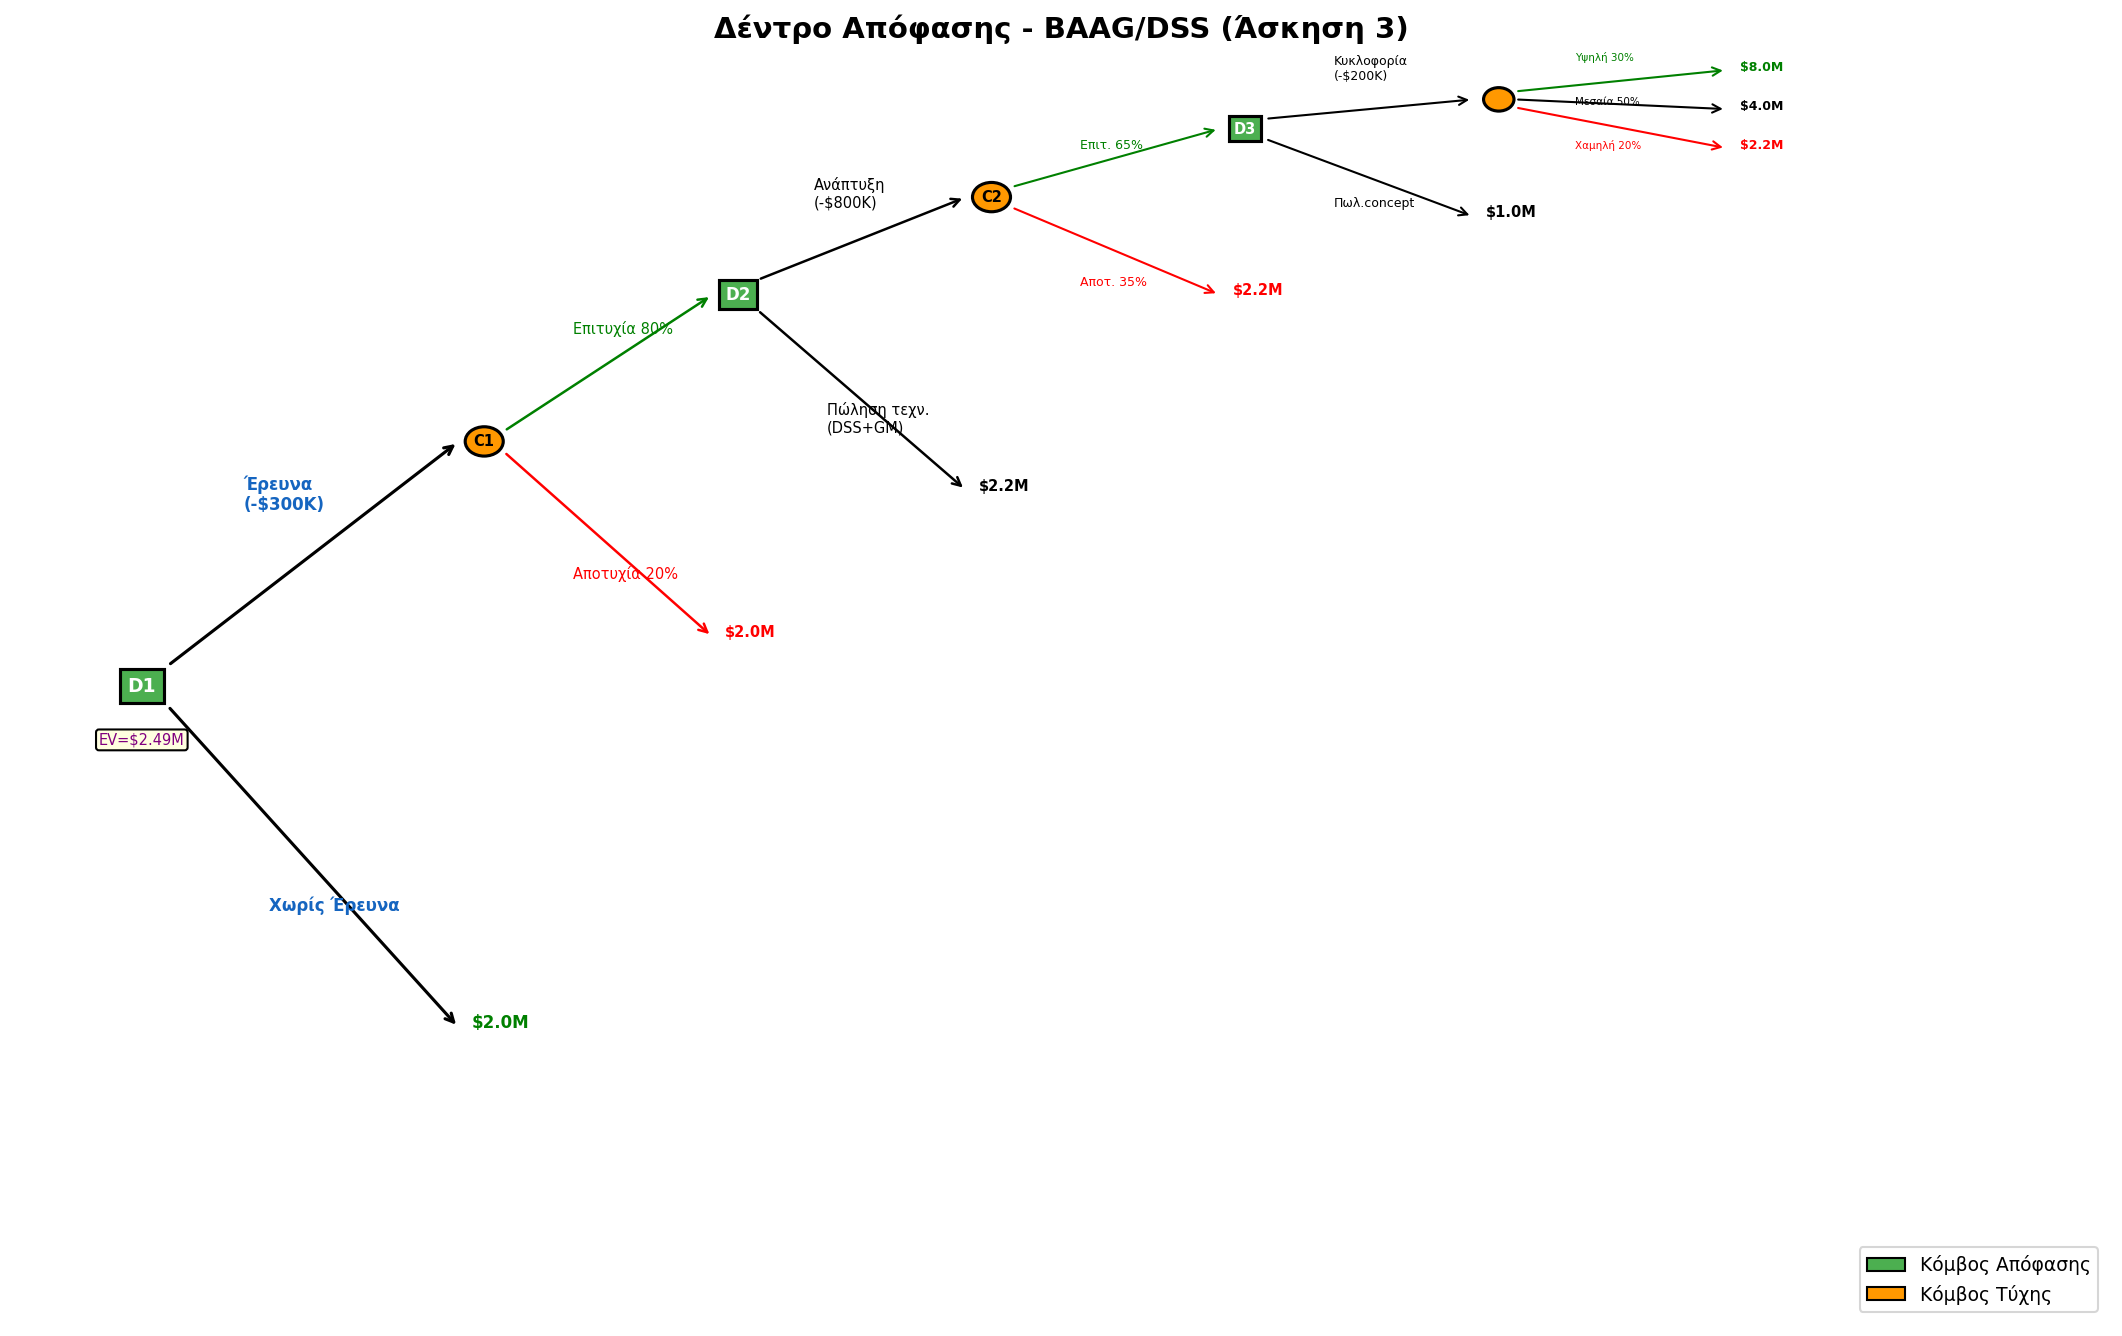
\includegraphics[width=\textwidth]{figures/ex3_baag_tree.png}
    \caption{Δέντρο Απόφασης -- BAAG/DSS}
\end{figure}


% ============================================================================
% ΑΣΚΗΣΗ 4: Carolina Cougars
% ============================================================================
\newpage
\section{The Carolina Cougars}

\subsection{Εννοιολογική Προσέγγιση}

Οι Carolina Cougars (ομάδα μπέιζμπολ) εξετάζουν τρεις στρατηγικές απόκτησης παικτών:
\begin{enumerate}
    \item \textbf{Καμία επένδυση} (\$0): 25\% πιθανότητα διεκδίκησης τίτλου
    \item \textbf{Μέτρια επένδυση} (\$20M): 50\% πιθανότητα διεκδίκησης
    \item \textbf{Μεγάλη επένδυση} (\$52M): 65\% πιθανότητα διεκδίκησης
\end{enumerate}

Κατά τη διάρκεια της σεζόν, η ομάδα μπορεί να αγοράσει/πωλήσει παίκτες ανάλογα με την πορεία της. Στόχος: μεγιστοποίηση αναμενόμενων κερδών.

\subsection{Μοντέλο και Λύση}

\subsubsection{Στρατηγική 1: Καμία Επένδυση}

\textbf{Αν Contender (25\%):}
\begin{align}
EV &= 0.70 \times 170 + 0.25 \times 115 + 0.05 \times 90 = 119 + 28.75 + 4.5 = \$152.25\text{M}
\end{align}

\textbf{Αν Out (75\%):}
\begin{align}
EV &= 0.05 \times 95 + 0.20 \times 55 + 0.75 \times 30 = 4.75 + 11 + 22.5 = \$38.25\text{M}
\end{align}

\begin{align}
EV(\text{S1}) = 0.25 \times 152.25 + 0.75 \times 38.25 = 38.0625 + 28.6875 = \mathbf{\$66.75\text{M}}
\end{align}

\subsubsection{Στρατηγική 2: Μέτρια Επένδυση (\$20M)}

\textbf{Contender (50\%):}
\begin{align}
EV(\text{Stand Pat}) &= 0.75 \times 195 + 0.20 \times 160 + 0.05 \times 120 = \$184.25\text{M} \\
EV(\text{Buy}) &= 0.80 \times 200 + 0.15 \times 170 + 0.05 \times 125 - 8 = \$183.75\text{M}
\end{align}
$\rightarrow$ \textbf{Stand Pat}: $\$184.25\text{M}$

\textbf{Out (50\%):}
\begin{align}
EV(\text{Stand Pat}) &= 0.12 \times 110 + 0.28 \times 65 + 0.60 \times 40 = \$55.40\text{M} \\
EV(\text{Sell} + \$8\text{M}) &= 0.08 \times 100 + 0.22 \times 60 + 0.70 \times 35 + 8 = \$53.70\text{M}
\end{align}
$\rightarrow$ \textbf{Stand Pat}: $\$55.40\text{M}$

\begin{align}
EV(\text{S2}) = 0.50 \times 184.25 + 0.50 \times 55.40 - 20 = \mathbf{\$99.83\text{M}}
\end{align}

\subsubsection{Στρατηγική 3: Μεγάλη Επένδυση (\$52M)}

\textbf{Contender (65\%):}
\begin{align}
EV(\text{Stand Pat}) &= 0.80 \times 210 + 0.15 \times 170 + 0.05 \times 125 = \$199.75\text{M} \\
EV(\text{Buy} - \$10\text{M}) &= 0.83 \times 220 + 0.12 \times 175 + 0.05 \times 130 - 10 = \$200.10\text{M}
\end{align}
$\rightarrow$ \textbf{Buy}: $\$200.10\text{M}$

\textbf{Out (35\%):}
\begin{align}
EV(\text{Stand Pat}) &= 0.15 \times 110 + 0.30 \times 70 + 0.55 \times 50 = \$65.00\text{M} \\
EV(\text{Sell} + \$12\text{M}) &= 0.10 \times 105 + 0.30 \times 65 + 0.60 \times 45 + 12 = \$69.00\text{M}
\end{align}
$\rightarrow$ \textbf{Sell}: $\$69.00\text{M}$

\begin{align}
EV(\text{S3}) = 0.65 \times 200.10 + 0.35 \times 69.00 - 52 = \mathbf{\$102.22\text{M}}
\end{align}

\subsubsection{Τελική Σύγκριση}

\begin{table}[H]
\centering
\begin{tabular}{lcr}
\toprule
\textbf{Στρατηγική} & \textbf{Κόστος} & \textbf{EV (\$M)} \\
\midrule
Καμία Επένδυση & \$0 & 66.75 \\
Μέτρια Επένδυση & \$20M & 99.83 \\
\textbf{Μεγάλη Επένδυση} & \textbf{\$52M} & \textbf{102.22} \\
\bottomrule
\end{tabular}
\caption{Σύγκριση στρατηγικών -- Carolina Cougars}
\end{table}

\begin{tcolorbox}[colback=green!10, colframe=decisiongreen, title=Βέλτιστη Πολιτική -- Carolina Cougars]
\begin{enumerate}
    \item \textbf{Μεγάλη Επένδυση (\$52M)} σε free agents
    \item Αν Contender (65\%) $\rightarrow$ \textbf{Αγορά παικτών} (-\$10M) κατά τη σεζόν
    \item Αν Out (35\%) $\rightarrow$ \textbf{Πώληση παικτών} (+\$12M)
\end{enumerate}
Αναμενόμενη αξία: \textbf{\$102.22M}
\end{tcolorbox}

\begin{figure}[H]
    \centering
    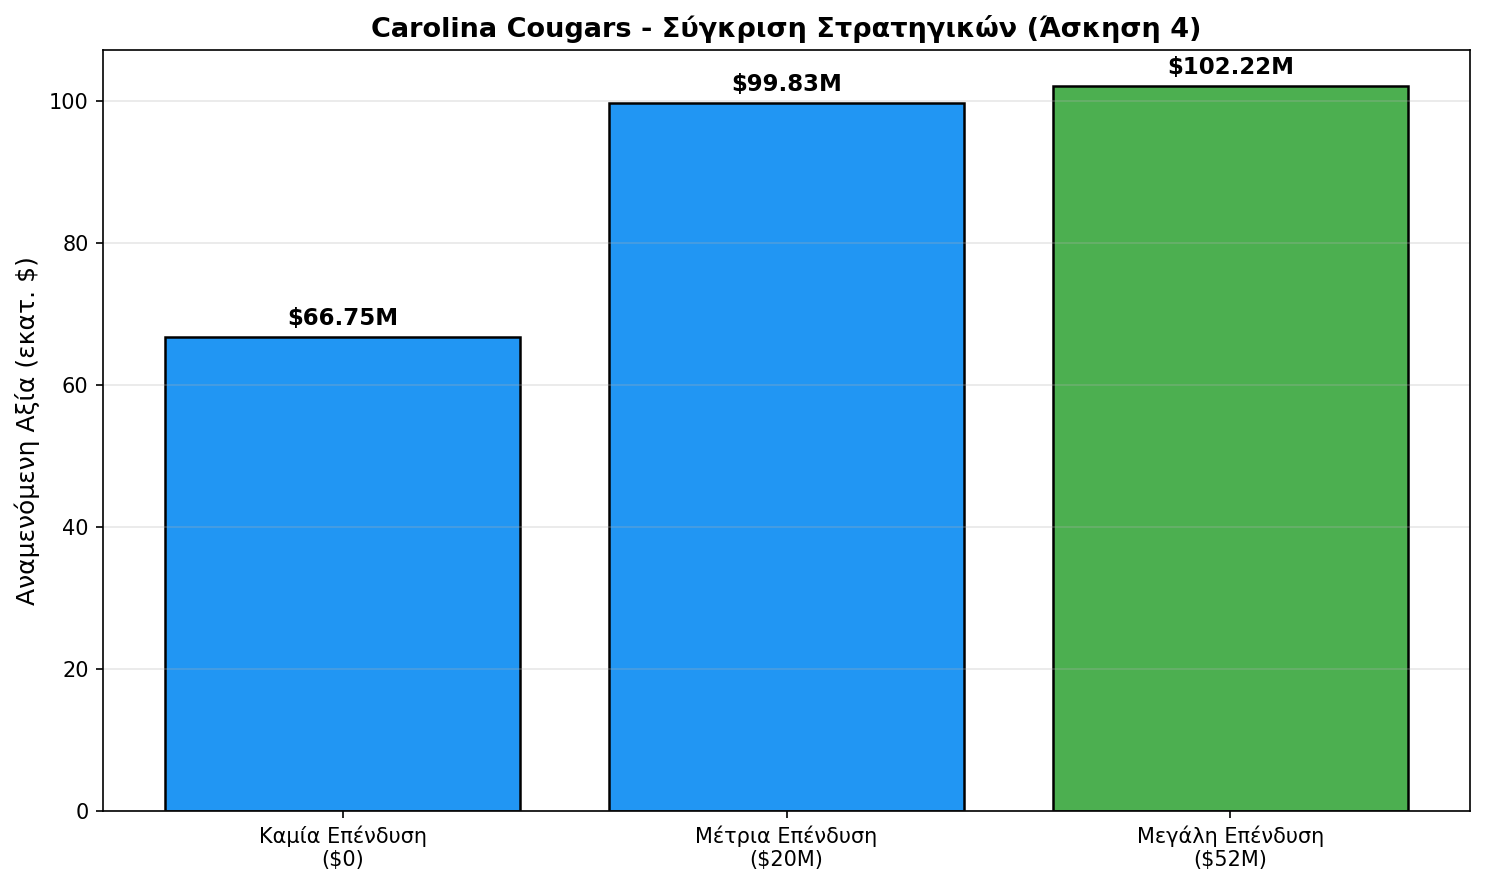
\includegraphics[width=\textwidth]{figures/ex4_cougars_comparison.png}
    \caption{Σύγκριση στρατηγικών -- Carolina Cougars}
\end{figure}

\begin{figure}[H]
    \centering
    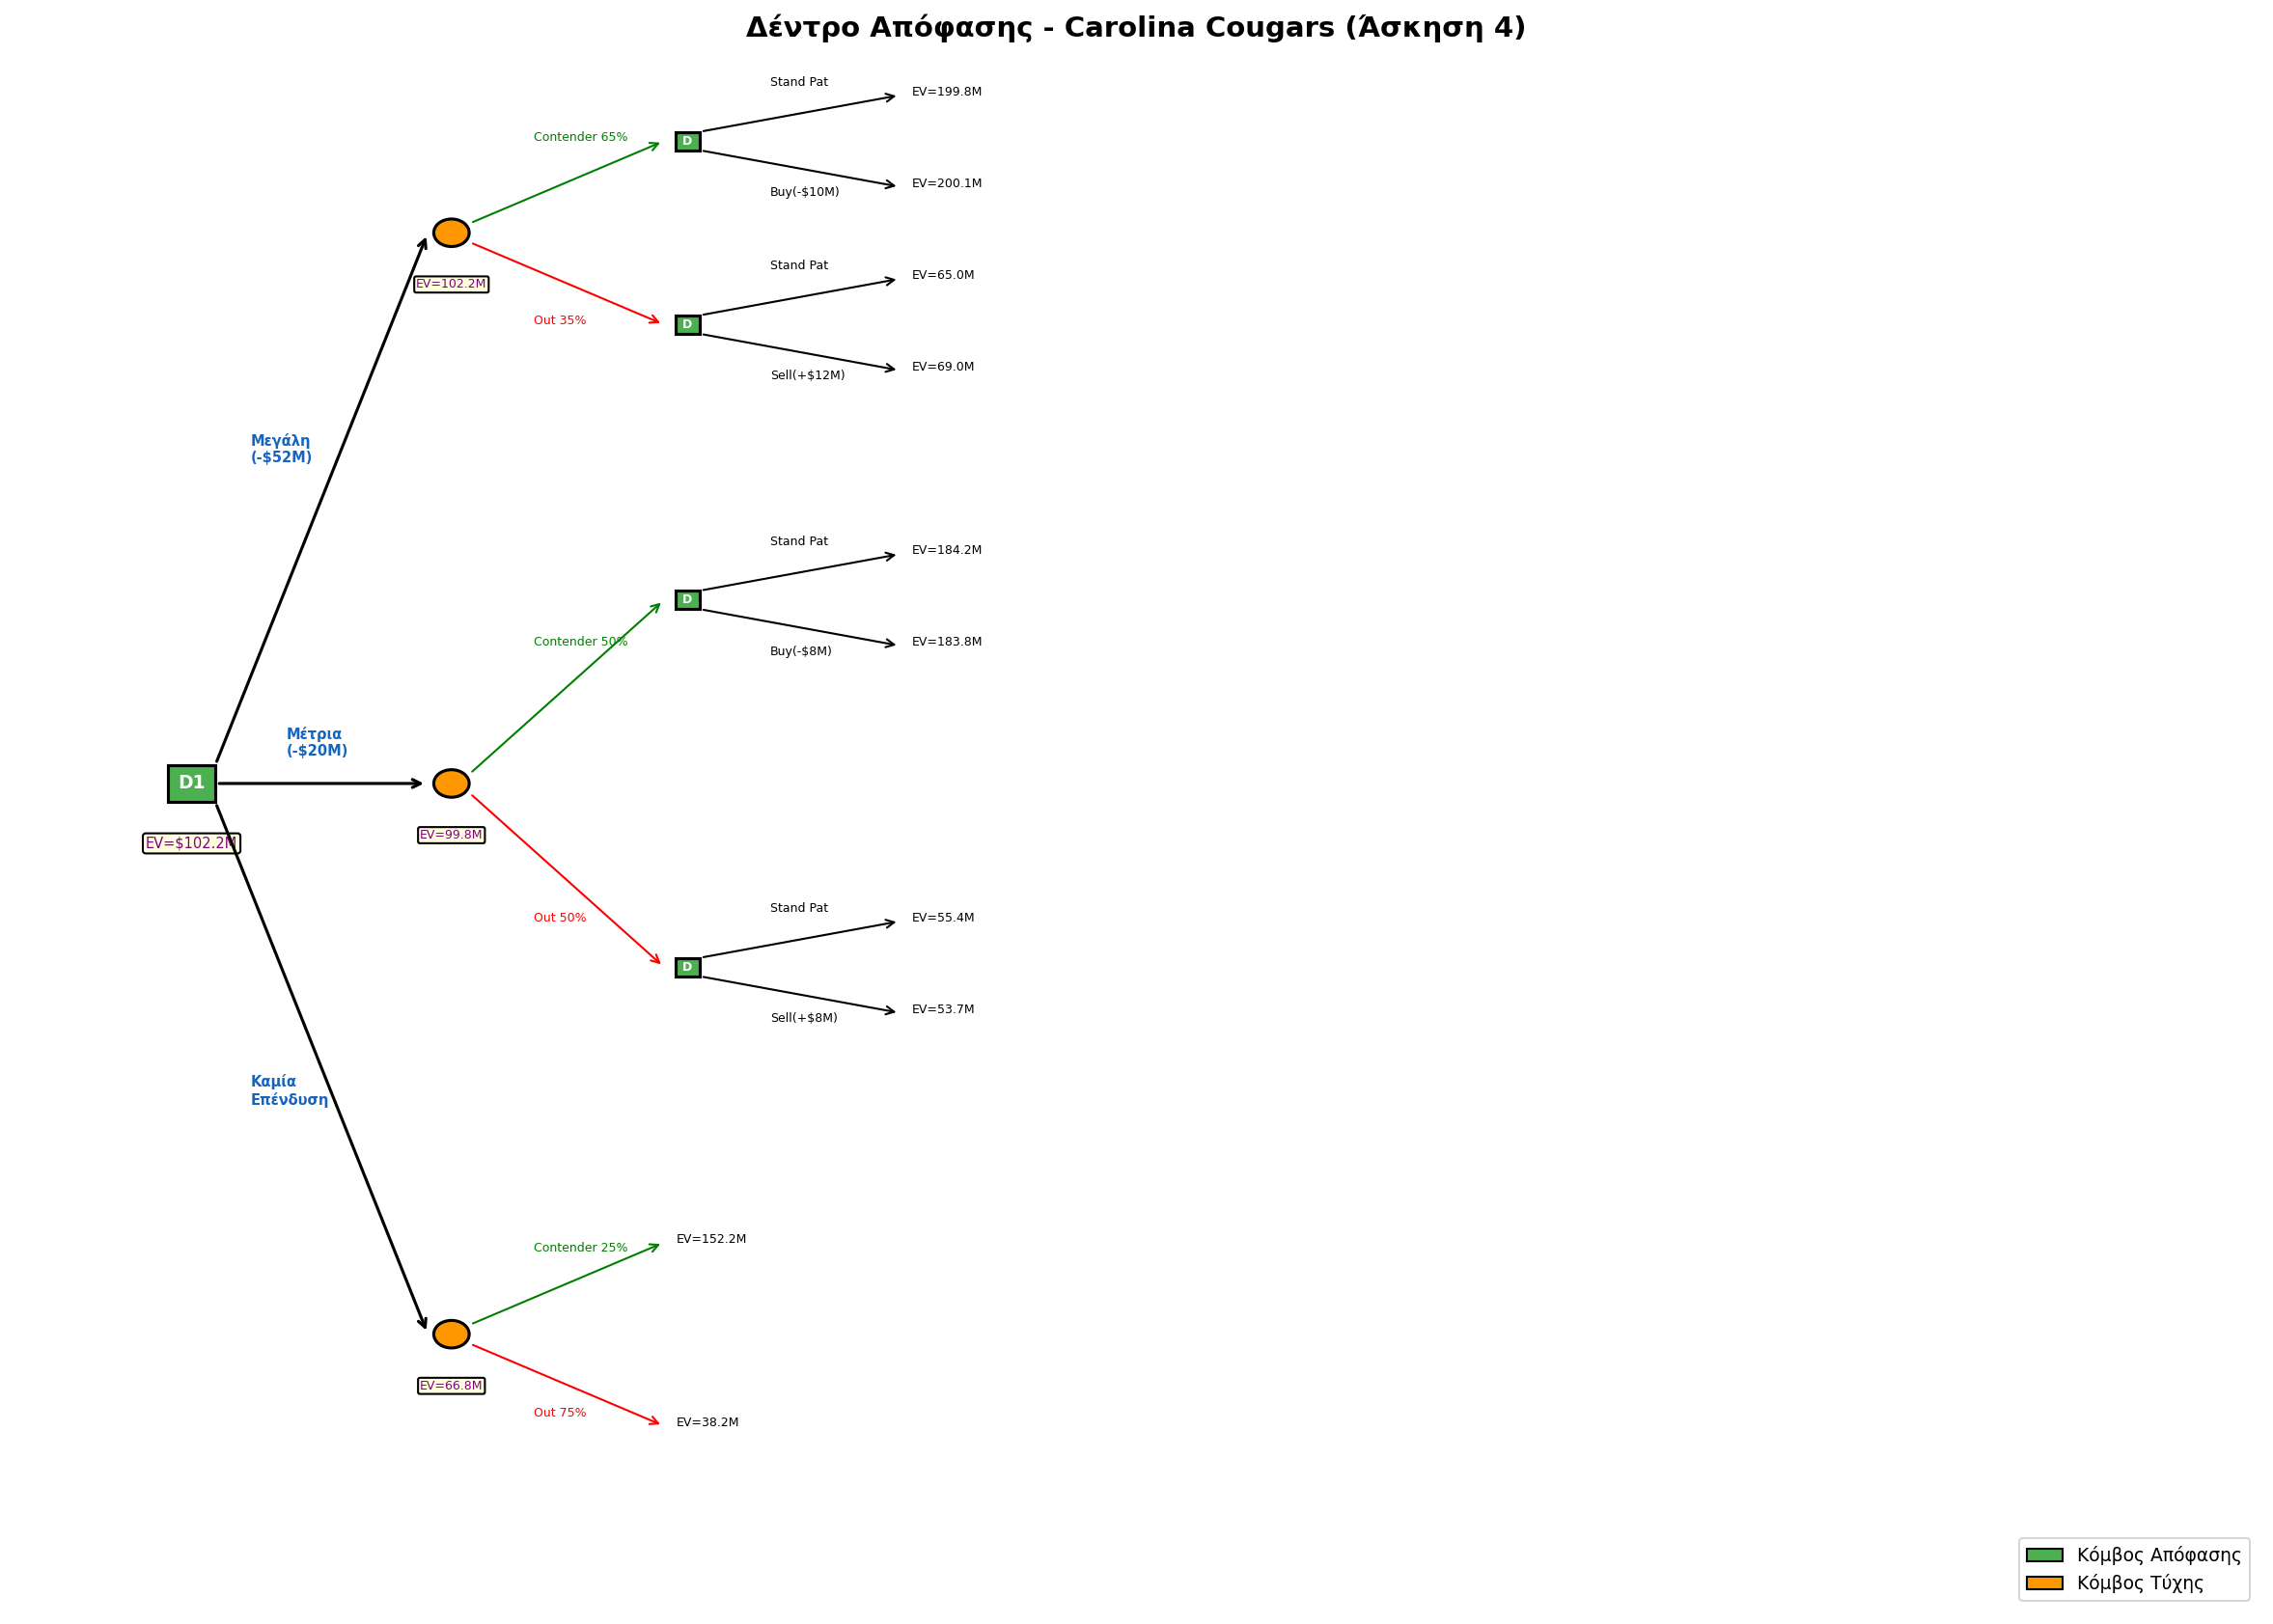
\includegraphics[width=\textwidth]{figures/ex4_cougars_tree.png}
    \caption{Δέντρο Απόφασης -- Carolina Cougars}
\end{figure}


% ============================================================================
% ΑΣΚΗΣΗ 5: Brainy Business
% ============================================================================
\newpage
\section{Brainy Business (Cerebrosoft)}

\subsection{Εννοιολογική Προσέγγιση}

Η Cerebrosoft εξετάζει την κυκλοφορία του λογισμικού Brainet. Το πρόβλημα περιλαμβάνει:
\begin{itemize}
    \item \textbf{Αβεβαιότητα ανταγωνισμού}: Σκληρός (20\%), Μέτριος (70\%), Ασθενής (10\%)
    \item \textbf{Εναλλακτικές τιμές}: \$50, \$40, \$30
    \item \textbf{Δυνατότητα}: Πρόσληψη εταιρείας έρευνας αγοράς (\$10,000)
    \item \textbf{Κόστος}: Ανάπτυξη \$800K + Ετήσια υποστήριξη \$50K
\end{itemize}

\subsection{Μέρος 1: Πίνακας Αποδοχών}

Η αποδοχή υπολογίζεται: $\text{Payoff} = \text{Τιμή} \times \text{Πωλήσεις} - \$800{,}000 - \$50{,}000$

\begin{table}[H]
\centering
\begin{tabular}{c|ccc}
\toprule
\textbf{Τιμή / Πωλήσεις} & \textbf{50,000} & \textbf{30,000} & \textbf{20,000} \\
\midrule
\$50 & \$1,650,000 & \$650,000 & \$150,000 \\
\$40 & \$1,150,000 & \$350,000 & -\$50,000 \\
\$30 & \$650,000 & \$50,000 & -\$250,000 \\
\bottomrule
\end{tabular}
\caption{Πίνακας Αποδοχών -- Cerebrosoft}
\end{table}

\textbf{Πιθανότητες πωλήσεων ανά ανταγωνισμό:} Οι πίνακες 1--3 από την εκφώνηση δίνουν τις πιθανότητες $P(\text{Πωλήσεις} \mid \text{Ανταγωνισμός}, \text{Τιμή})$.

\subsection{Μέρος 2: Κανόνας Bayes}

Η αναμενόμενη αποδοχή υπολογίζεται ως:
\begin{align}
EV(\text{Τιμή}) = \sum_{c} P(c) \sum_{s} P(s \mid c, \text{Τιμή}) \times \text{Payoff}(s, \text{Τιμή})
\end{align}

Όπου $c \in \{\text{Σκληρός, Μέτριος, Ασθενής}\}$ και $s \in \{50\text{K}, 30\text{K}, 20\text{K}\}$.

\textbf{Αναλυτικός υπολογισμός για $\$50$:}
\begin{align}
EV(\$50) &= 0.20 \times [0.20(1{,}650{,}000) + 0.25(650{,}000) + 0.55(150{,}000)] \nonumber \\
&+ 0.70 \times [0.25(1{,}650{,}000) + 0.30(650{,}000) + 0.45(150{,}000)] \nonumber \\
&+ 0.10 \times [0.30(1{,}650{,}000) + 0.35(650{,}000) + 0.35(150{,}000)] \nonumber \\
&= 0.20 \times 575{,}000 + 0.70 \times 675{,}000 + 0.10 \times 775{,}000 \nonumber \\
&= 115{,}000 + 472{,}500 + 77{,}500 = \mathbf{\$665{,}000}
\end{align}

\begin{table}[H]
\centering
\begin{tabular}{lr}
\toprule
\textbf{Στρατηγική} & \textbf{EV (\$)} \\
\midrule
\textbf{Τιμή \$50} & \textbf{665,000} \\
Τιμή \$40 & 470,000 \\
Τιμή \$30 & 252,500 \\
Εγκατάλειψη & 0 \\
\bottomrule
\end{tabular}
\caption{Αναμενόμενες αποδοχές χωρίς έρευνα αγοράς}
\end{table}

\begin{tcolorbox}[colback=blue!10, colframe=resultblue, title=Απόφαση Bayes (χωρίς έρευνα)]
Η Charlotte πρέπει να \textbf{κυκλοφορήσει το Brainet στα \$50} με αναμενόμενη αποδοχή \textbf{\$665,000}.
\end{tcolorbox}

\subsection{Μέρος 3: Έρευνα Αγοράς}

\subsubsection{Αξιοπιστία Εταιρείας Έρευνας (Likelihood)}

\begin{table}[H]
\centering
\begin{tabular}{l|ccc}
\toprule
\textbf{Πραγματικός} $\backslash$ \textbf{Πρόβλεψη} & Σκληρός & Μέτριος & Ασθενής \\
\midrule
Σκληρός & 0.80 & 0.15 & 0.05 \\
Μέτριος & 0.15 & 0.80 & 0.05 \\
Ασθενής & 0.03 & 0.07 & 0.90 \\
\bottomrule
\end{tabular}
\caption{Πίνακας αξιοπιστίας έρευνας αγοράς}
\end{table}

\subsubsection{Υπολογισμός Posterior Πιθανοτήτων (Θεώρημα Bayes)}

\textbf{Βήμα 1: Πιθανότητα κάθε πρόβλεψης}
\begin{align}
P(\text{Πρ.Σκλ.}) &= 0.20(0.80) + 0.70(0.15) + 0.10(0.03) = 0.160 + 0.105 + 0.003 = 0.268 \\
P(\text{Πρ.Μετ.}) &= 0.20(0.15) + 0.70(0.80) + 0.10(0.07) = 0.030 + 0.560 + 0.007 = 0.597 \\
P(\text{Πρ.Ασθ.}) &= 0.20(0.05) + 0.70(0.05) + 0.10(0.90) = 0.010 + 0.035 + 0.090 = 0.135
\end{align}

\textbf{Βήμα 2: Posterior πιθανότητες}

Εφαρμόζοντας τον τύπο Bayes: $P(A_i \mid B) = \frac{P(B \mid A_i) P(A_i)}{P(B)}$

\begin{table}[H]
\centering
\begin{tabular}{l|ccc}
\toprule
\textbf{Posterior} & $P(\cdot \mid \text{Πρ.Σκλ.})$ & $P(\cdot \mid \text{Πρ.Μετ.})$ & $P(\cdot \mid \text{Πρ.Ασθ.})$ \\
\midrule
Σκληρός & 0.5970 & 0.0503 & 0.0741 \\
Μέτριος & 0.3918 & 0.9380 & 0.2593 \\
Ασθενής & 0.0112 & 0.0117 & 0.6667 \\
\bottomrule
\end{tabular}
\caption{Posterior πιθανότητες ανταγωνισμού}
\end{table}

\subsubsection{EV ανά Πρόβλεψη}

\begin{table}[H]
\centering
\begin{tabular}{l|rrr}
\toprule
\textbf{Πρόβλεψη} & \textbf{EV(\$50)} & \textbf{EV(\$40)} & \textbf{EV(\$30)} \\
\midrule
Σκληρός ανταγ. & \$616,418 & \$424,030 & \$216,063 \\
Μέτριος ανταγ. & \$671,147 & \$467,856 & \$257,111 \\
Ασθενής ανταγ. & \$734,259 & \$570,741 & \$304,444 \\
\midrule
\textbf{Βέλτιστη} & \textbf{\$50} & --- & --- \\
\bottomrule
\end{tabular}
\caption{EV ανά πρόβλεψη και τιμή}
\end{table}

Σε \textbf{κάθε} πρόβλεψη, η τιμή \$50 είναι βέλτιστη και θετική.

\subsubsection{Αξία Έρευνας Αγοράς}

\begin{align}
EV(\text{Με Έρευνα}) &= P(\text{Πρ.Σκλ.}) \times EV^*(\text{Πρ.Σκλ.}) + P(\text{Πρ.Μετ.}) \times EV^*(\text{Πρ.Μετ.}) \nonumber \\
&\quad + P(\text{Πρ.Ασθ.}) \times EV^*(\text{Πρ.Ασθ.}) - \$10{,}000 \nonumber \\
&= 0.268 \times 616{,}418 + 0.597 \times 671{,}147 + 0.135 \times 734{,}259 - 10{,}000 \nonumber \\
&= 165{,}200 + 400{,}675 + 99{,}125 - 10{,}000 = \mathbf{\$655{,}000}
\end{align}

\begin{tcolorbox}[colback=green!10, colframe=decisiongreen, title=Βέλτιστη Πολιτική -- Cerebrosoft]
\textbf{Δεν αξίζει η πληρωμή \$10,000 για έρευνα αγοράς.}
\begin{itemize}
    \item $EV(\text{Χωρίς Έρευνα}) = \$665{,}000 > EV(\text{Με Έρευνα}) = \$655{,}000$
    \item Η πληροφορία από την έρευνα δεν αλλάζει τη βέλτιστη απόφαση σε κανένα σενάριο (πάντα \$50)
    \item \textbf{Η Charlotte πρέπει να κυκλοφορήσει το Brainet στα \$50 χωρίς έρευνα}
\end{itemize}
Αναμενόμενη αποδοχή: \textbf{\$665,000}
\end{tcolorbox}

\begin{figure}[H]
    \centering
    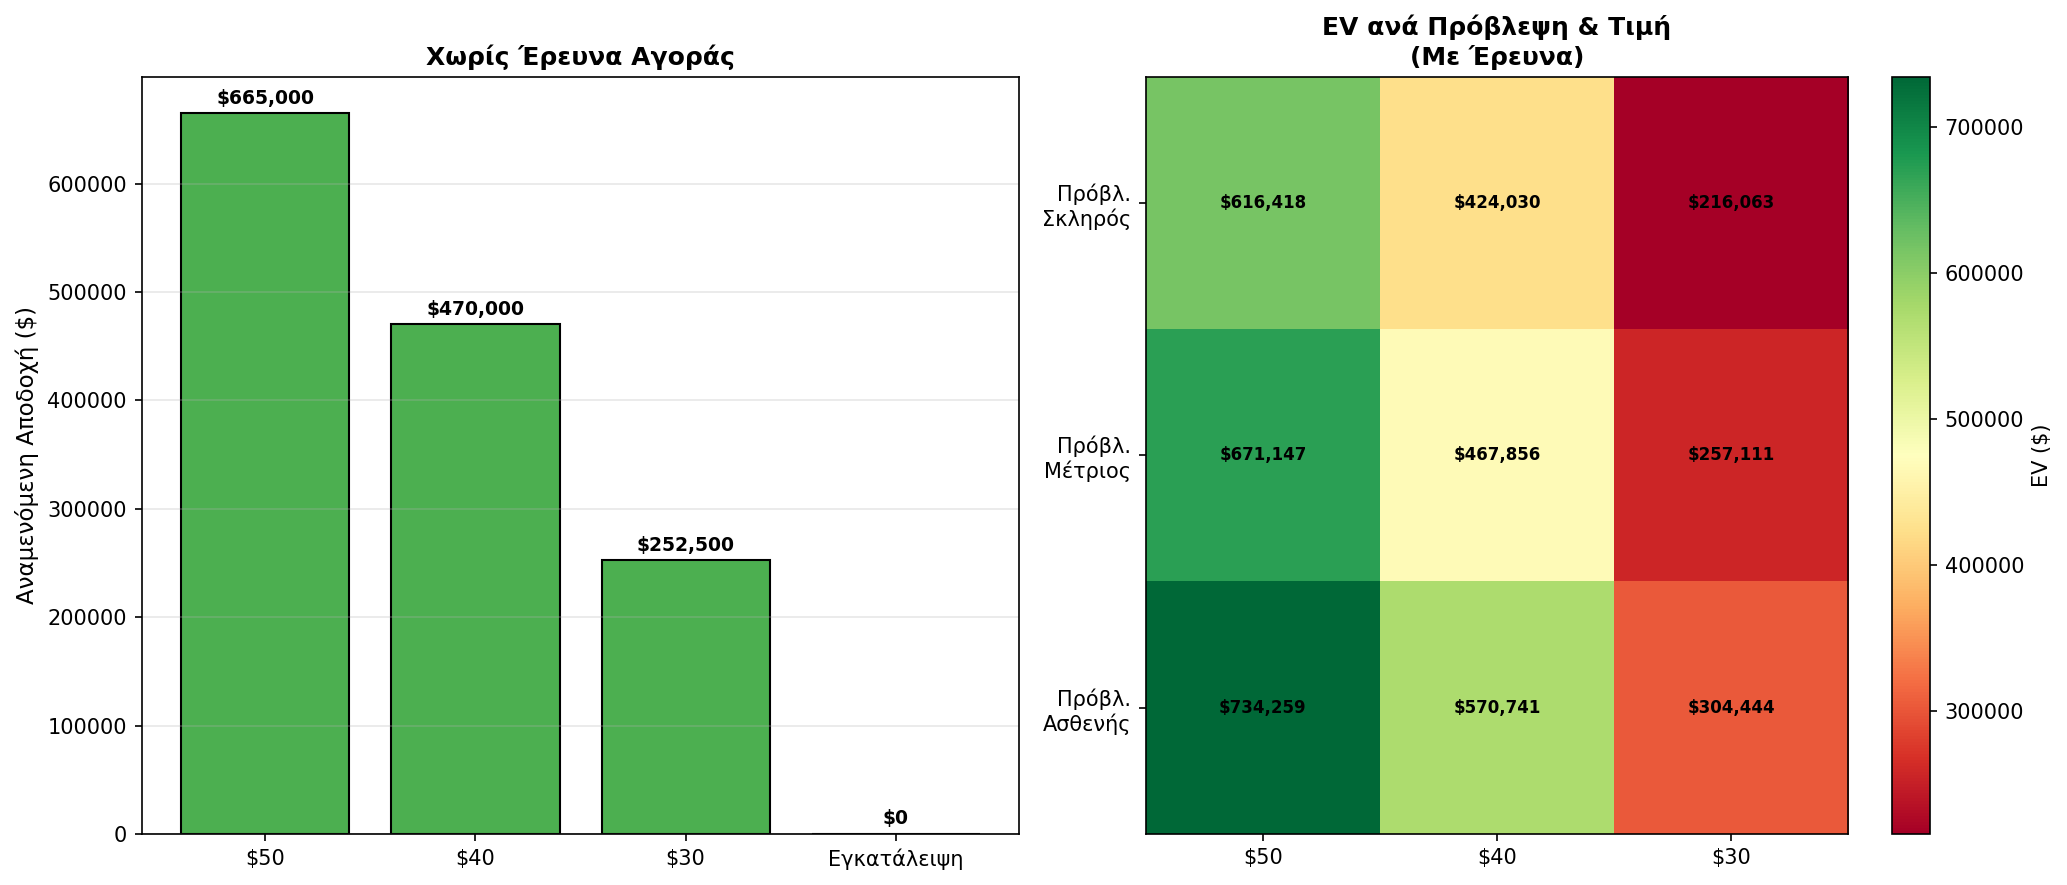
\includegraphics[width=\textwidth]{figures/ex5_cerebrosoft.png}
    \caption{Ανάλυση αποδοχών Cerebrosoft -- Χωρίς \& Με Έρευνα}
\end{figure}

\begin{figure}[H]
    \centering
    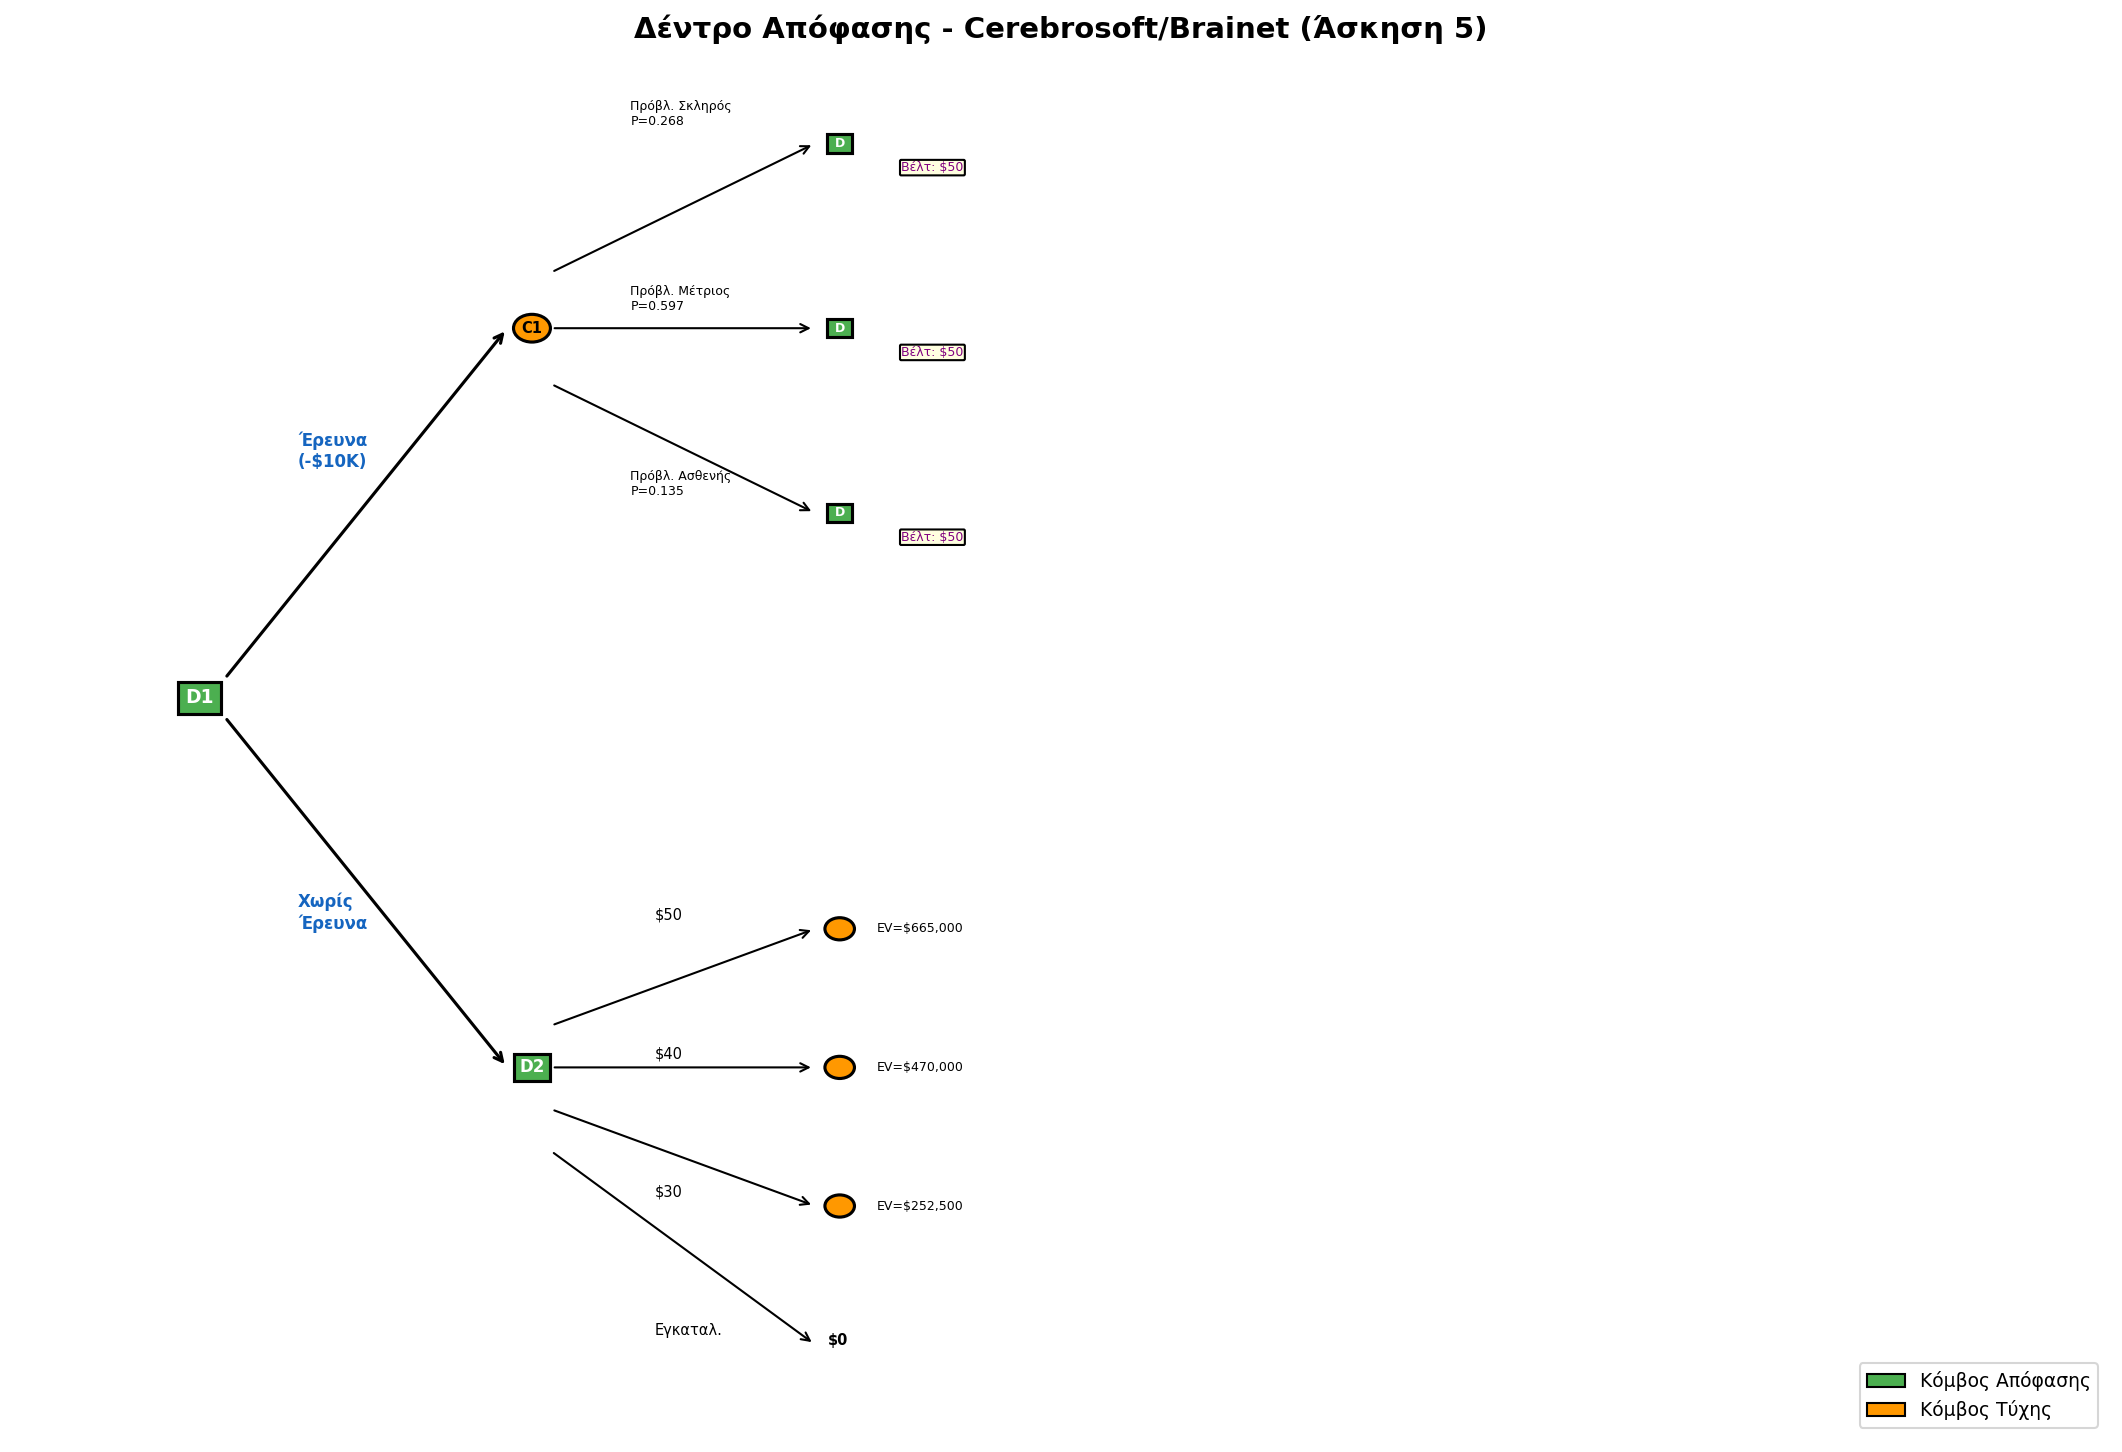
\includegraphics[width=\textwidth]{figures/ex5_cerebrosoft_tree.png}
    \caption{Δέντρο Απόφασης -- Cerebrosoft}
\end{figure}

% ============================================================================
% ΑΝΑΦΟΡΕΣ
% ============================================================================
\newpage
\section*{Αναφορές Λογισμικού}

\begin{itemize}
    \item \textbf{Python 3}: Van Rossum, G. \& Drake, F.L., 2009. \textit{Python 3 Reference Manual}. CreateSpace.
    \item \textbf{NumPy}: Harris, C.R. et al., 2020. Array programming with NumPy. \textit{Nature}, 585(7825), pp.357--362.
    \item \textbf{Matplotlib}: Hunter, J.D., 2007. Matplotlib: A 2D graphics environment. \textit{Computing in Science \& Engineering}, 9(3), pp.90--95.
    \item Ολοι οι υπολογισμοί πραγματοποιήθηκαν με κώδικα Python (αρχείο \texttt{solution.py}).
\end{itemize}

\end{document}
